\documentclass[a4paper,11pt]{article}
\usepackage[latin1]{inputenc}
\usepackage[T1]{fontenc}
\usepackage{amsmath}
\usepackage{a4wide}
\usepackage{booktabs}
\usepackage{graphicx}
\usepackage{url}

\title{Genomics and Bioinformatics}
\date{October 30, 2012}
\author{Exam correction}
\begin{document}
\maketitle

\section*{Question 1 - Sequence Alignment}

\subsection*{Linear gap penalty}

\begin{figure}[h]
\centering\includegraphics[scale=.4]{scoring_matrix.png}
\end{figure}

the four optimal alignments are below:

\begin{verbatim}
ATTCCGTTA  ATTCCGTTA  ATTCCGTTA  ATTCCGTTA
AT--CG--A  AT-C-G--A  A-T-CG--A  A-TC-G--A
\end{verbatim}

\subsection*{Affine gap penalty}

All alignments have $5$ matches and $4$ gaps. The first has $2$ gap
openings, hence a score of,
$$
5\times 2-4\times 1-2\times 2\,=\,2~,
$$
the other three have $3$ gap openings, with a score of:
$$
5\times 2-4\times 1-3\times 2\,=\,0~.
$$


\section*{Question 2 - Phylogenetic trees}

\begin{enumerate}

\item The tree:

\centering
\includegraphics[width=0.6\textwidth]{phylo.png}\\

\item 
\begin{itemize}
	\item A pair of orthologs: mm\_ins1, rn\_ins1
	\item A pair of parologs from the same species: mm\_ins1, mm\_ins2
	\item A pair of parologs from different species: rn\_ins1, mm\_ins2
\end{itemize}

\end{enumerate}

Here is the reference document and the complete tree (duplications in red):

\vspace{0.5cm}
\centering
\includegraphics[width=0.9\textwidth]{phylo2.png}
\vspace{0.3cm}

\url{http://www.ncbi.nlm.nih.gov/pmc/articles/PMC2652215/}


\section*{Question 3 - Genome Assembly}

\begin{enumerate}

\item
\begin{figure}[h]
\centering\includegraphics[scale=.5]{Hamilton.pdf}
\end{figure}

The Hamiltonian path starts with the blue arrow and generates the
following contig:\\
CCATGCATGCCATGTC

\item 
The 4-mers and 5-mers sets are:
\begin{eqnarray*}
  S_4 &=& \{\mbox{CCAT,CATG,ATGC,TGCA,GCAT,TGCC,GCCA,ATGT,TGTC}\}.\\
  S_5&=&\{\mbox{CCATG,CATGC,ATGCA,} \\
  &&\phantom\{\mbox{TGCAT,GCATG,CATGC,} \\
  &&\phantom\{\mbox{ATGCC,TGCCA,GCCAT,} \\
  &&\phantom\{\mbox{CCATG,CATGT,ATGTC}\}.
\end{eqnarray*}


\item The de Bruijn graph is as below:
\begin{figure}[h]
\centering\includegraphics[scale=.5]{Brujin.pdf}
\end{figure}

\item 
The green edge in the figure above makes the graph eulerian,
possible paths are\\
\small{CCAT-CATG-ATGC-TGCA-GCAT-CATG-ATGC-TGCC-GCCA-CCAT-CATG-ATGT-TGTC}\\
\small{CCAT-CATG-ATGC-TGCC-GCCA-CCAT-CATG-ATGC-TGCA-GCAT-CATG-ATGT-TGTC }\\
\normalsize{leading to two possible contigs}:\\
CCATGCATGCCATGTC \\
CCATGCCATGCATGTC \\

The second contig does not contain the read TGCATGC (for example).
\end{enumerate}

\section*{Question 4 - HMMs}

\begin{center}
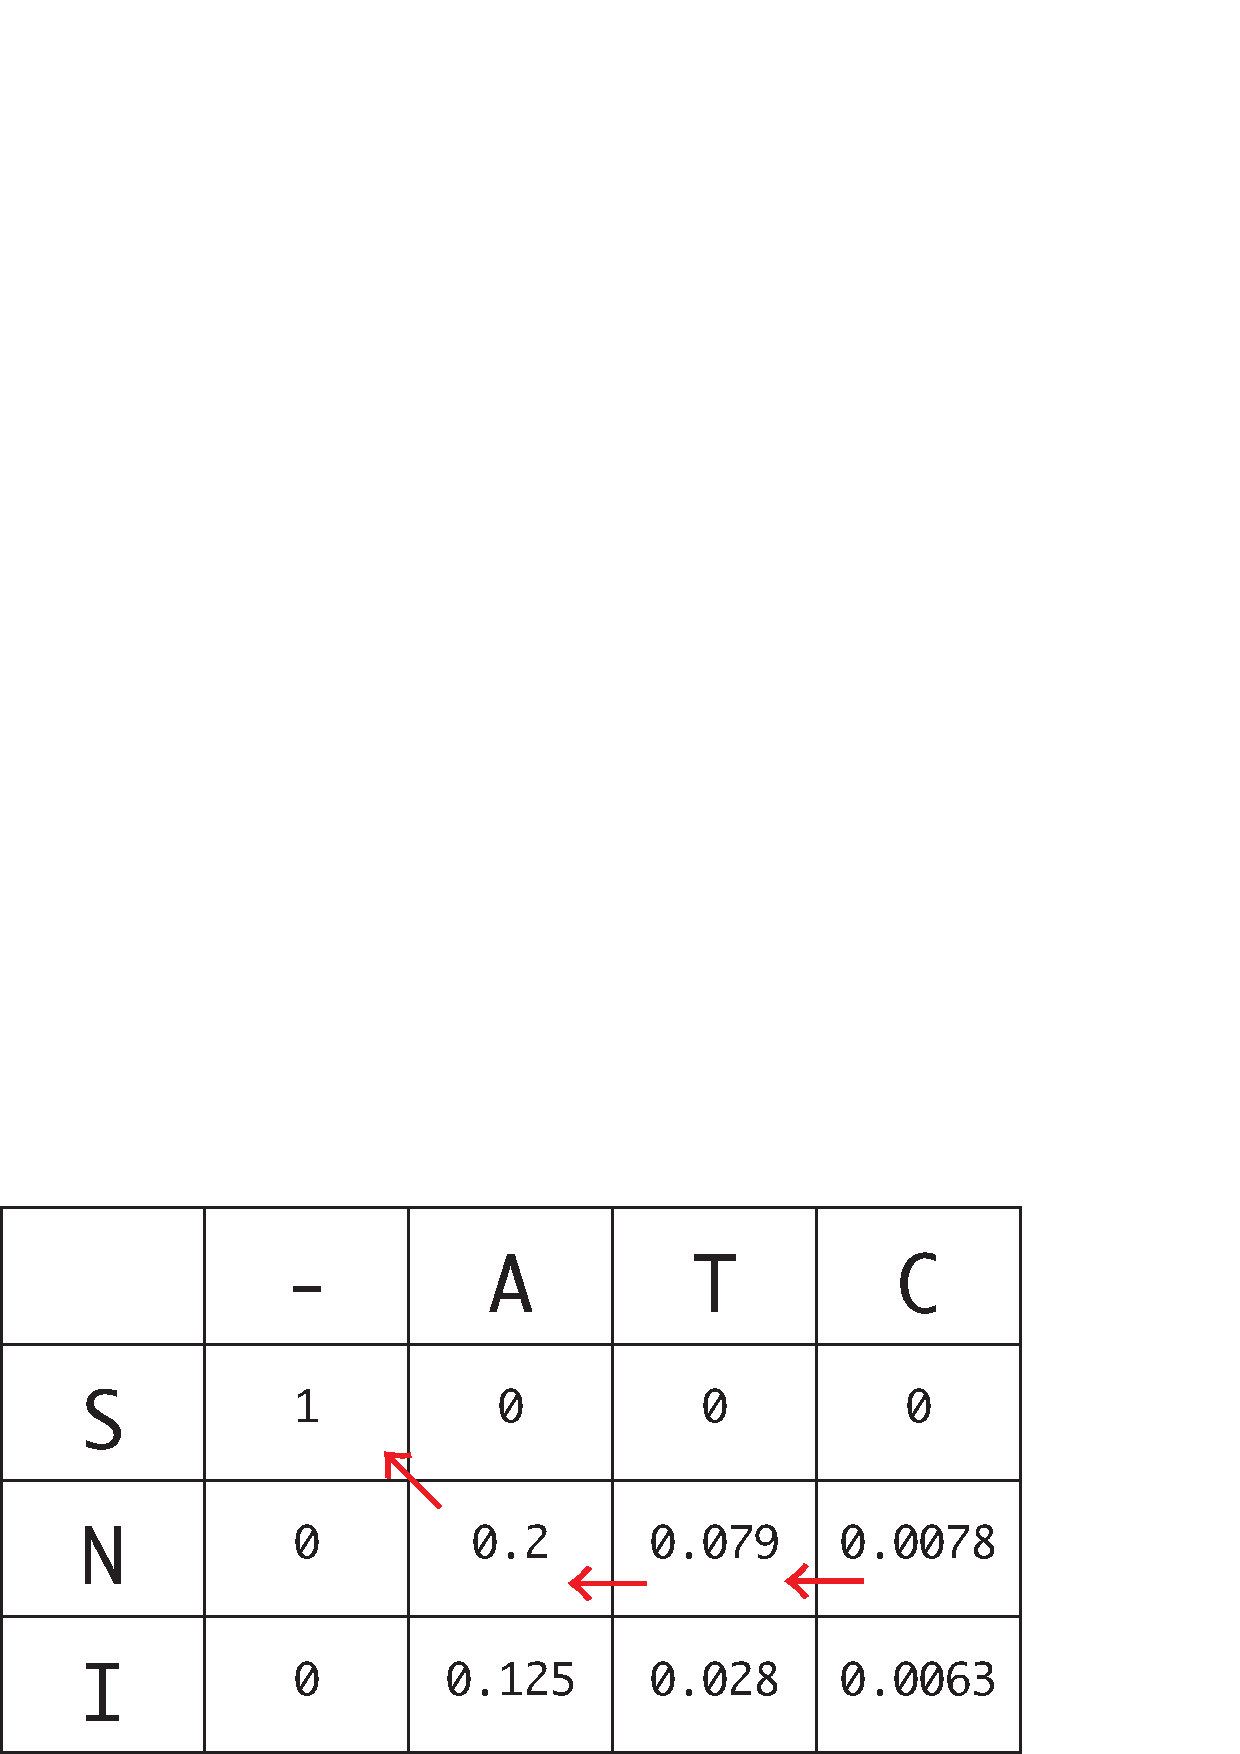
\includegraphics[scale=.5]{fig3.pdf}\\
\end{center}
The most probable hidden sequence associated to CGA is XYX.

\end{document}
